
\section{信号検出}

\subsection{必要な同期制度のための信号検出の要件}

精密な測距・時刻同期のためには精密な信号検出が必要である.
まず許容される信号検出の誤差について考える,

スマートデバイスのサンプリング周波数を44100Hz
として
1サンプルあたりの時間解像度は約 1/44100 = 22.6μs
であるので,
1サンプルあたりの距離解像度は 22.6μs*340m/s=7.7mm(音速340m/sと仮定)
である.

人間の聴覚特性として,第一波面の法則という現象が知られている\cite{Haas}.
これは二つの音源からの音声が互いに50ms以上ずれると別の音源として知覚されるというものである.

この場合許容される誤差は
$\pm$ 50msの誤差におよそ $\pm$ 2205サンプル以内とかなり緩いものになる.
しかしこれでは距離誤差が $\pm$ 3.4m となり,教室空間での位置推定のパラメータとして使うにはとても大きなものになってしまう.
そのため,許容される誤差は音像定位ではなく距離測定の手法によって定められるといえる.
室内空間であれば,
$\pm$ 50cmの誤差つまり $\pm$ 64サンプル以内でパルスを同定できればよいとする.


\subsection{本研究で試したパルス圧縮の種類}

本研究で試行したパルス圧縮を表 \ref{tab:pulsecomps} にまとめる.

\begin{table}[p]\centering
  \caption{本研究で試したパルス圧縮の種類}
  \label{tab:pulsecomps}
  \begin{tabular}{ll|ccc}
    \hline
    パルス & 利点 & 欠点 \\
    \hline
    \parbox{10zw}{固定周波数パルス}
      & \parbox{10zw}{可聴域外のパルスに設定可能}
      & \parbox{10zw}{ノイズに弱い,ピーク発見が困難, \\ 可聴域外音声の発生・受信が安価な端末では困難}
      \\
    \hline
    \parbox{10zw}{全帯域チャープ信号}
      & \parbox{10zw}{パルス圧縮によりノイズに強い}
      & \parbox{10zw}{信号強度確保のために \\ 持続時間を長くするとピークが鈍くなる}
      \\
    \hline
    \parbox{10zw}{バーカー符号を用いた \\ 直接スペクトル拡散}
      & \parbox{10zw}{鋭いピークを持たせられる}
      & \parbox{10zw}{系列長が13までしかないため \\ SN比に限界がある}
      \\
    \hline
    \parbox{10zw}{バーカー符号化\\ チャープ信号}
      & \parbox{10zw}{短いチャープをバーカー符号化することで \\ チャープのピークを鋭く保ったまま13倍にできる}
      & \parbox{10zw}{高周波数帯の非線形歪みの影響で \\ 複数のピークが現れる}
      \\
    \hline
    \parbox{10zw}{M系列を用いた\\ 直接スペクトル拡散}
      & \parbox{10zw}{パルス持続時間を伸ばしてSN比を高めてもピークが鋭い}
      & \parbox{10zw}{持続時間を長くしすぎると非線形歪みの影響で \\ 複数のピークが現れる}
      \\
    \hline
  \end{tabular}
\end{table}

まず可聴域外に近い20000Hz前後の固定周波数パルスを用いた同期信号を試みた.
しかし,安価なスマートデバイスのスピーカとアンプとマイクロホンでは送受信ができない,
可聴域音にしても信号の検出が困難などの理由で不採用となった.

次に,チャープ信号を用いたパルス圧縮手法を試みた.
これにより信号強度を高める事ができた.
だが,信号のサイドローブが大きく鋭いピークを持たせられなかった.

チャープ信号に代わるもとして,バーカー符号を用いた直接スペクトル拡散を考えたが,
バーカー符号は系列長13までしかないので,そのまま直接拡散してもパルス持続時間が短くSN比を向上できない.
そこで,直接拡散において符号化する1波長を通常の正弦波ではなくひとつのチャープ信号にするパルス圧縮信号を試みた.
しかし,これも高周波数帯域の非線形歪みの影響を受け,複数のピークが現れた.

最後に,M系列符号を用いた直接スペクトル拡散を試みた.
これにより,ピークを鋭く保ったまま任意の持続時間のパルスを作ることができるようになった.
しかし,持続時間をむやみに長くすると,非線形歪みの影響を受けるようになった.

これらを順に説明する.

\subsection{固定周波数パルス}

本研究ではまず固定周波数パルスを試みた.
周波数を可聴域外に近い20000Hz前後にすることで,
利用者の耳には聞こえにくい同期信号を利用できると考えたからである.
これは実際MacBookProなどの高品質な端末では送受信可能だったが,
Nexus7(2013)などの比較的安価な端末のスピーカやマイクでは送受信できなかった.
また,この信号は可聴域としてもピークが鈍くで同期信号には適さなかった.

\subsection{チャープ信号}

そこで,チャープ信号を用いたパルス圧縮を試みた.
チャープ信号は時間に対して周波数を変化させた信号で,
同じ長さの固定周波数パルスに対してピークを鋭くすることができる利点がある.
しかし.持続時間を長くするとピークが鈍くなってしまう.
これによりマルチパスの影響により現れる複数のピークが重なってしまい,最初に届いた波のピークを特定することを困難とさせていた.
このため,この同期・測距信号には適さなかった.

\subsection{バーカー符号化チャープ信号}

そこでさらに,バーカー符号とチャープ信号のふたつのパルス圧縮方式を組み合わせる独自のパルス圧縮を考案した\cite{self_ac}.
バーカー符号とチャープ信号の二つのパルス圧縮技術を組み合わせて,チャープ信号をバーカー符号を用いてBPSKで変調したものである.
バーカー符号は直接スペクトル拡散方式で用いられる拡散系列で,
Diracのデルタ関数に近いするどい相関特性を持つ.
しかし,このようなパルスは系列長13までしか存在しないので,そのまま直接拡散しても持続時間を長くできずSN比を向上させられない.
そこで,バーカー符号を用いてBPSKして直接拡散するにあたって,チップ幅を1波長の正弦波ではなく,ひとつのチャープ信号を用いる事で,
チャープ信号の鋭さを保ったまま通常のチャープ信号の13倍のSN比を稼げると考えた
(図\ref{fig:barker_chirp},\ref{fig:barker_coded_chirp},\ref{fig:barker_coded_chirp_err},\ref{fig:corr}).

\begin{figure}[p]\centering
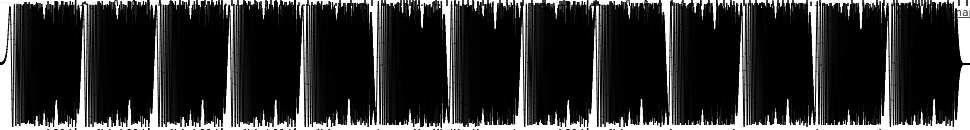
\includegraphics[clip,width=1.0\hsize]{img/barker_chirp.png}
\caption{チャープ信号を搬送波として長さ13のバーカー符号でBPSK変調信号したもの}\label{fig:barker_chirp}
\end{figure}

\begin{figure}[p]\centering
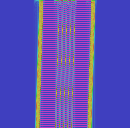
\includegraphics[clip,width=0.75\hsize]{img/barker_coded_chirp.png}
\caption{チャープ信号を搬送波として長さ13のバーカー符号でBPSK変調信号したもののスペクトルグラム(シミュレーション)}\label{fig:barker_coded_chirp}
\end{figure}


\begin{figure}[p]\centering
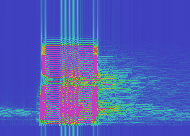
\includegraphics[clip,width=0.75\hsize]{img/barker_coded_chirp_err.png}
\caption{チャープ信号を搬送波として長さ13のバーカー符号でBPSK変調信号したもののスペクトルグラム
(MacBookAirによる実環境での自身の信号の計測結果)}\label{fig:barker_coded_chirp_err}
\end{figure}



\begin{figure}[p]\centering
\vspace{2mm}
\begin{small}
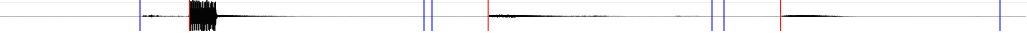
\includegraphics[clip,width=1.0\hsize]{img/rawdata.png}\\
A端末自身のパルス~ ~ ~ ~
B端末のパルス~ ~ ~ ~ ~
C端末のパルス\\\vspace{0.5mm}
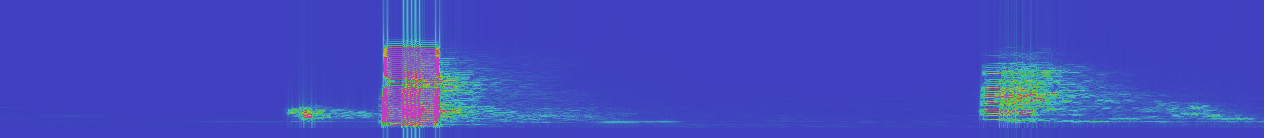
\includegraphics[clip,width=0.8\hsize]{img/spectrogram.png}\hspace{1cm}\\
A端末自身のパルス~ ~ ~ ~ ~ ~ ~ ~ ~
B端末のパルス\\\vspace{0.5mm}
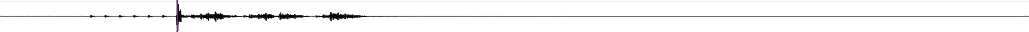
\includegraphics[clip,width=1.0\hsize]{img/corrA.png}\\
A端末のパルスに整合フィルタをかけたもの\\\vspace{0.5mm}
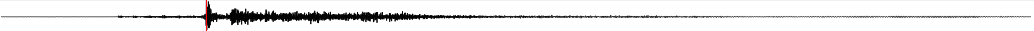
\includegraphics[clip,width=1.0\hsize]{img/corrB.png}\\
B端末のパルスに整合フィルタをかけたもの\\\vspace{0.5mm}
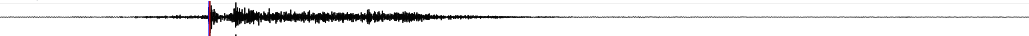
\includegraphics[clip,width=1.0\hsize]{img/corrC.png}\\
C端末のパルスに整合フィルタをかけたもの\\
\vspace{1mm}
\caption{A端末で観測したABC端末のパルス信号}\label{fig:corr}

\end{small}
\vspace{1mm}
\end{figure}

提案手法のパルス圧縮に関して,
以前利用していたこのバーカー符号化チャープ信号によるパルス圧縮ではなく,
M系列符号による直接拡散方式を用いた理由について以下で述べる.

本来barker codeはそのままサイン波に適用し直接拡散して使うものであるが,
系列長が最大で13までしかないため,パルス圧縮に上限があった.
一方でチャープ信号は引き伸ばせば引き伸ばすほどパルス圧縮されるが,サイドローブが大きくなるという問題を抱えていた.
そのため,この二つの手法を組み合わせて,短いup-chirpの繰り返しをbarker codeで拡散することで,
サイドローブを抑えながら圧縮する手法を試みた.
しかし,この手法は高周波成分において非線型歪みの影響を受けやすく,複数のピークが現れてしまうという問題を抱えていた.
%要図

一方で,M系列符号には系列長に制限がないため,そのような手法を必要とせず,直接拡散方式が利用できる.
%以前の実装は私がbarker codeによるパルス圧縮を知った時点で,まだM系列符号を知らなかった故のものであり,
%M系列符号が使える現在,そのようなハイブリット手法を使う理由はない.





\subsection{M系列による直接スペクトル拡散}

本研究ではM系列符号による直接スペクトル拡散方式によるパルス圧縮を用いた.
これはチャープ信号よりも非定常雑音に強い\cite{nonlinear}.
また,信号検出には通常の整合フィルタではなくピークを尖らせることができる,
フェイズオンリー整合フィルタ(phase-only matched filter: POF)\cite{pof, phaseonly2}を利用した(図\ref{fig:pof}).
フェイズオンリー整合フィルタは,整合フィルタに信号の周波数成分のみを利用することでサイドローブを抑えピークをとがらせることができるフィルタである.

\begin{figure}[p]\centering
  \hspace{-2mm}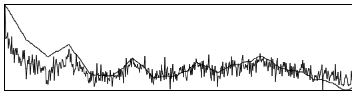
\includegraphics[clip,width=1.1\hsize]{img/POF.png}
  \caption{フェイズオンリー整合フィルタと整合フィルタ}\label{fig:pof}
\end{figure}

$$
\begin{aligned}
\mathrm{POF}[x_a, x_b]
&= \mathcal{F}^{-1}\left[\frac{\mathcal{F}\left[x_a(t)\right]^*}{|\mathcal{F}\left[x_a(t)\right]|}\mathcal{F}\left[x_b(t)\right]\right] \\
&= \mathcal{F}^{-1}\left[\frac{X_a^*(\omega)}{|X_a(\omega)|}X_b(\omega)\right]
\end{aligned}
$$


直接スペクトル拡散方式(direct sequence spread spectrum:DSSS)(図\ref{fig:DS})による測距システムの変復調方式を図\ref{fig:DME2}に示す.
搬送波には4410Hz正弦波を,拡散符号には符号長1023のM系列を用い,変調にはバイナリ位相シフトキーイング(BPSK)を使った.

\begin{figure}[p]\centering
  \hspace{-2mm}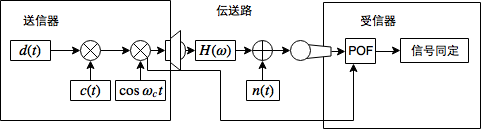
\includegraphics[clip,width=1.1\hsize]{img/DME2.png}
  \caption{変復調システム図}\label{fig:DME2}
\end{figure}

\begin{figure}[p]\centering
  \hspace{-2mm}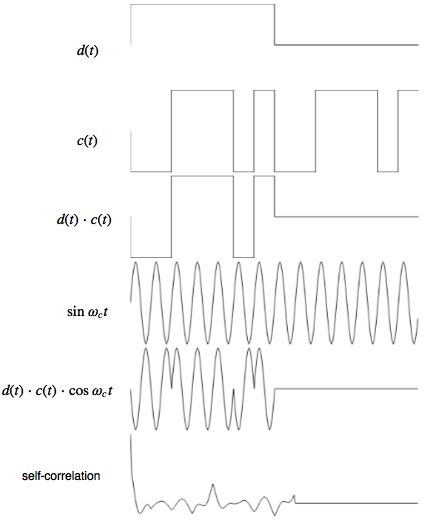
\includegraphics[clip,width=1.1\hsize]{img/DSSS.png}
  \caption{直接スペクトラム拡散による信号変調過程}\label{fig:DSSS}
\end{figure}

この手法により,通常のパルスやチャープ信号,バーカー符号化チャープよりも鋭くSN比の高いピークが得られるようになった.
しかし,まだ問題は残っており,継続時間を長くしすぎると送受信側のシステムクロックのずれにより非線形歪みの影響を受け,ピークが複数現れるようになってしまう.
そこで



\subsection{伝送路推定用の参照信号を用いた信号同定}

復調した受信信号が雑音か有効な信号かを決定する処理を信号同定という.
伝送路における伝達関数 $H(\omega)$ において室内残響の影響
としてマルチパスによる影響を受けてしまう(図\ref{fig:multipath}).

\begin{figure}[p]\centering
  \hspace{-2mm}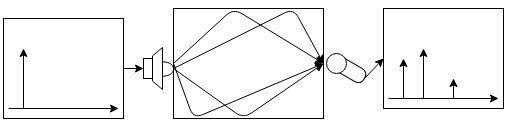
\includegraphics[clip,width=1.1\hsize]{img/multipath.png}
  \caption{反射波・回折波によるマルチパスの影響}\label{fig:multipath}
\end{figure}


そこで,同期パルスを測距用信号と,伝搬路を測定する参照波の二つに分離した.
参照波を用いた伝送路推定にはCDMA通信でのRake受信器において使われているサウンダ信号や,
OFDM通信などではパイロット信号が推定信号として使われる.
同期パルスから $n$ 秒後に参照信号を送り,
その二つの信号の相関を取ることで,
背景雑音とは別にパルス位置を特定することが可能になる(図\ref{fig:sounder}).

\begin{figure}[p]\centering
  \hspace{-2mm}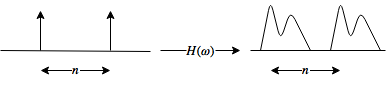
\includegraphics[clip,width=1.1\hsize]{img/sounder.png}
  \caption{同期信号と参照信号}\label{fig:sounder}
\end{figure}

さらに参照信号と測距信号は互いに異なる同周期のM系列を用いた.
参照信号と測距信号を判別しやすくするためである.

この時刻が $n$ 秒ずれた二つの信号に対して時間窓で区切って相互相関をとることで,
信号が最も相関している区間,つまり信号の位置を特定することができる.
最後に,その区間相関値を閾値処理することで信号の到来を決定する.
今回は最大相関値前方での40\%の相関値を超えたピークを到来時刻としている.

相関関数の計算には Wiener-Khintchine の定理を使い,周波数領域での複素乗算としてFFTを使って計算することで計算量を減らすことができる.
長さの異なる信号の高速フーリエ変換には重畳加算法\cite{overwrap}を使った.


\begin{figure}[p]
  \centering
  \includegraphics[clip,width=1.05\hsize]{img/026.jpeg}
  \caption{変復調回路}\label{fig:henpuku}
\end{figure}


\begin{figure}[p]
  \centering
  \includegraphics[clip,width=1.05\hsize]{img/029.jpeg}
  \caption{信号同定過程}\label{fig:shousai}
\end{figure}




\clearpage
